\subsection{Compiler's limitation, and how to bypass them}

The compiler’s strategy of partitioning the iteration space into blocks $128 \times 128 \times 128$, supplemented by a 4-way unroll-and-jam transformation, is explicitly engineered to maximize the utilization of the  memory hierarchy. 

With those implementation choices, a single $128 \times 128$ tile of requires 128 KB of memory. While this exceeds the 48 KB L1D cache capacity, the \emph{unroll-and-jam} allow for sub-tiles to stay in L1D, while the full $128 \times 128$ block fits inside the L2 cache (1.25 MB per core). 

However, this hardware-specific optimization counld falls short in practice, due to a fundamental limitation in the cache implementation (Behavioral details of the Associative Caches are discussed in Appendix~\ref{subsec:caching}). 

\subsubsection{Cache Collisions in Matrix Traversal}
For simplicity, we consider an aligned matrix implementation with cache-line padding (i.e., the starting pointer is cache-aligned, and the matrix content is perfectly bounded by cache lines): under those constrains, we can find the worst-case scenario of cache trashing.

When iterating through a matrix column, the CPU accesses addresses separated by the length of an entire matrix row. If this row length in memory exactly matches the distance between \emph{cache sets}, the first element of every row will map to the exact same, causing severe cache thrashing by evicting one of the already-allocated cache lines\footnote{Usually the cache eviction follows a Least-Recently-Used (LRU) replacement policy, hence will be removed the cache line first addressed.}.

For a cache with a power-of-two number of sets, addresses map to the same set if they are separated by exactly $2^{(\text{Set bits} + \text{Offset bits})}$ bytes. For a matrix of double-precision floating-point numbers (\texttt{sizeof(double)} $= 8$ bytes), the required row length to force a collision is:
$$ \text{Row Length} = \frac{2^{(\text{Set bits} + \text{Offset bits})}}{8} \text{ elements} $$

Based on the hardware specifications in Table~\ref{tab:cache_partitioning}, we can calculate the exact matrix dimensions that trigger these set collisions:

\begin{itemize}
    \item \textbf{L1 Cache Collision:} 
    The L1 cache uses 6 Offset bits and 6 Set bits.
    $$ \text{L1 Distance} = 2^{(6 + 6)} = 2^{12} \text{ bytes} = 4096 \text{ bytes} $$
    $$ \text{L1 Row Length} = \frac{4096}{8} = 512 \text{ elements} $$
    If the matrix has exactly 512 columns (or a multiple of it), the first element of every row maps to the same L1 set. Since the L1 is 12-way associative, reading just 13 rows in a column will completely fill the set and force an eviction of the first row (as observed in Figure~\ref{fig:icc_icx_aligned_comparison}).

    \item \textbf{L2 Cache Collision:}
    The L2 cache uses 6 Offset bits and 11 Set bits.
    $$ \text{L2 Distance} = 2^{(11 + 6)} = 2^{17} \text{ bytes} = 131,072 \text{ bytes} $$
    $$ \text{L2 Row Length} = \frac{131072}{8} = 16,384 \text{ elements} $$
    If the matrix has exactly 16,384 columns, column-major traversal will rapidly thrash the 10-way associative L2 cache.
\end{itemize}

\paragraph{Quantitative comparison}
This limitation can be verified by the in-depth study we completed by using Intel Advisor on the same ICX build (\texttt{-O3 -xHost -DALIGN}), testing both $N = 4096$ and $N=5000$.

\begin{figure}[H]
\centering
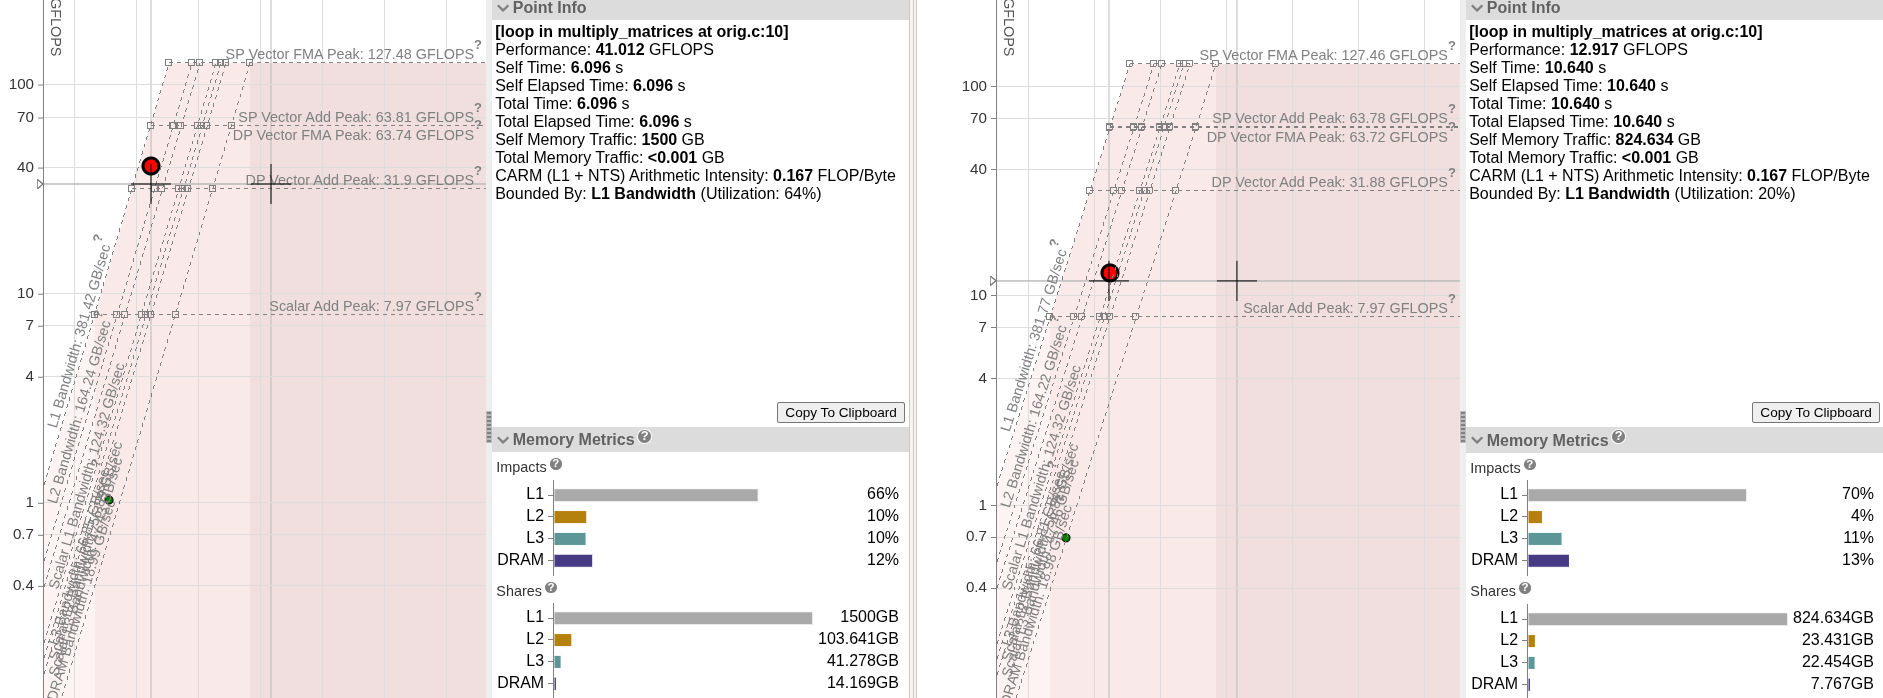
\includegraphics[width=1\textwidth]{Images/icx_4096_vs_5000.png}
\caption{Roofline model of \texttt{ICX -O3 -xHost -DALIGN} on \texttt{n=5000} and \texttt{n=4096}}
\label{fig:icc_icx_aligned_roofline_comparison}
\end{figure}


The highlighted bottlenecks are in both cases the L1, but we can clearly see a difference in their bandwidth utilization and overall performance impact. For the bigger matrix ($N=5000$), the L1 cache is utilized efficiently at 64\% of its peak bandwidth, allowing a performance of \textbf{41.01 GFLOPS}.

In contrast, the problematic one ($N=4096$) suffers a drop  to just \textbf{12.91 GFLOPS}. 

Despite executing fewer total mathematical operations (due to the smaller size), its L1 bandwidth utilization drops to a mere 20\%: this low utilization indicates that the CPU pipeline is heavily stalled waiting for data due to continuous cache conflict evictions (thrashing).



\subsubsection{Cache-Aware Solutions, to Dimension-Dependent Thrashing}

The cache thrashing problem  maximized by power-of-two matrices can be mitigated using three (alternative or complementary) strategies:

\begin{itemize}
    \item \textbf{Memory Padding:} extending each matrix row with a adequate number of cells (zeroed or inaccessible).
    By artificially forcing the row length to a non-power-of-two size\footnote{is possible to compute a runtime a heuristic matrix size that minimize problem, but for brevity purposes we will not explore those solutions.}, the memory addresses are staggered. 
    This naturally shift the column elements across different cache sets rather than concentrating them into the same one. 
    
    We discard this solution because it wastes significant memory space. Furthermore, it assumes we have full control over the original matrices allocations, which is rarely true in real-case scenarios.\footnote{Note that this differs from the minor cache-line alignment padding introduced earlier; padding to break L1 set collisions requires way larger, system-dependent offsets.}

    \item \textbf{Compile-Time Constant Dimensions:} The second solution relies on aggressive compiler optimization. When the matrix dimension $N$ is provided as a constant at compile time, the compiler can further mitigate the effect by using \emph{register blocking} (scalar replacement). Instead of repeatedly fetching conflicting addresses from the L1 cache, the compiler loads the active working set directly into the CPU's vector registers and holds them there throughout the inner loop's execution. 
    
    As shown in Table~\ref{tab:results_placeholder}, the compiler's knowledge partially mitigate the problem, but without completely removing it.

    \begin{table}[H]
    \centering
    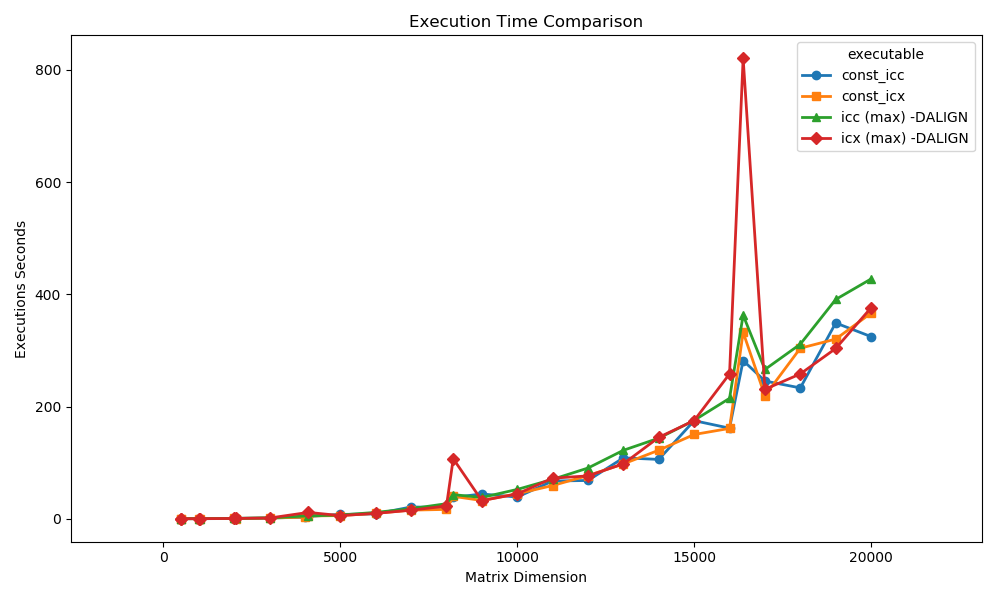
\includegraphics[width=0.8\textwidth]{Images/icc_icx_const.png}
    \caption{Performance comparison demonstrating the furhter dumping of cache thrashing spikes when $N$ is known at compilation time.}
    \label{tab:results_placeholder}
    \end{table}

    \item \textbf{Data Packing (Auxiliary Buffers):} The Last solution proposed is a technique widely employed by high-end optimization libraries such as \texttt{\texttt{OpenBLAS}}, whose detailed breakdown is provided in Appendix~\ref{subsec:openblas}. 
    
    The core idea is to explicitly allocate auxiliary memory buffers and manually copy the active tiles from matrices A and B into these buffers before computing them. Because these temporary matrices are strictly contiguous, they map cleanly across all available cache sets, completely bypassing the original column-stride layout. If implemented correctly and with suitable tile's dimensions, the time used to copy the tiles  will be largely repaid by the performance gains.
\end{itemize}

In the following section, we will present a custom, ad-hoc implementation that applies this packing strategy.
